\documentclass[leqno,10pt]{article}
\usepackage{boxedminipage}

\usepackage{html}

\html{ \newcommand{\bbm}{\vspace{5pt}\par\noindent\begin{boxedminipage}{2.0\linewidth}} }
\latex{ \newcommand{\bbm}{\vspace{5pt}\par\noindent\begin{boxedminipage}{1.05\linewidth}} }

% links to the maxima manual. this also gives the top directory
%\def\maxdocdir{/usr/share/doc/maxima-doc/html/}
%\def\maxdocdir{../maxima_html/}
\def\maxdocdir{http://maxima.sourceforge.net/docs/manual/en/}
\newcommand{\maxlink}[1]{{\maxdocdir}#1}
%\newcommand{\maxman}[2]{{\htmladdnormallink{#1}{{\maxdocdir}#2}}  % link to page in manual
\html{\newcommand{\maxman}[2]{\hlink{#1}{\maxlink{#2}}}}
\latex{\newcommand{\maxman}[2]{#1}}

\newcommand{\hlink}[2]{\htmladdnormallink{#1}{#2}}


\usepackage{graphicx}
\usepackage{hyperref}
%\usepackage{pdftex} % not there
%\usepackage{mathpazo}
%% following is added by imaxima output
\usepackage{verbatim}
\usepackage[cmbase]{flexisym}
\usepackage{bbold}

%bbold above conflicts with amssymb \usepackage{amssymb}
\usepackage{breqn}
\setkeys{breqn}{compact}

\def\supertiny{ \font\supertinyfont = cmr6 at 4pt \relax
\supertinyfont}

\usepackage{makeidx} 
\makeindex

%\usepackage{amssymb} this breaks bbold numeral
%\usepackage{amsmath}

\newcommand{\ebm}{\end{boxedminipage}\vspace{5pt}\par\noindent}
\setlength{\fboxrule}{0.1pt} 
\setlength{\fboxsep}{10pt}


\setlength{\textwidth}{180mm}
\setlength{\oddsidemargin}{15mm}
\addtolength{\oddsidemargin}{-1in}
\setlength{\evensidemargin}{15mm}
\addtolength{\evensidemargin}{-1in}

\newcommand{\ifrac}[2]{\frac{#1}{#2}}
\newcommand{\ifracd}[2]{\frac{#1}{#2}}
\newcommand{\ifracn}[2]{\frac{#1}{#2}}
\newcommand{\isubscript}[2]{{#1}_{#2}}
\newcommand{\iexpt}[2]{{#1}^{#2}}
\newcommand{\isqrt}[1]{\sqrt{#1}}
%% end lines added by imaxima output

\newcommand{\ket}[1]{{\lvert#1 \rangle}}
\newcommand{\bra}[1]{{\langle#1 \rvert}}
\newcommand{\func}[2]{{\bf #1}($#2$)}
\newcommand{\marray}[2]{{\bf #1}[$#2$]}
\newcommand{\fs}[1]{{\bf #1}}

% refer to a function and add an index entry
\newcommand{\ifs}[1]{{\bf #1}\index{#1@{\bf #1}}} % bold index entry plus bold in text
\newcommand{\ibd}[1]{\index{#1@{\bf #1}}} % bold index entry
\newcommand{\iit}[1]{\index{#1@{\it #1}}} % italic index entry
% package or software proper name, with an index entry
\newcommand{\ipname}[1]{{\it #1}\index{#1@{\it #1}}}
\newcommand{\pname}[1]{{\it #1}} % software name 
\newcommand{\imarray}[2]{\marray{#1}{#2}\index{#1@{\marray{#1}{#2}}}} % \marray with index entry
\newcommand{\ifunc}[2]{\func{#1}{#2}\index{#1@\func{#1}{#2}}} % \func with index entry
\newcommand{\qinf}{ {\it qinf } } % the name of this package
\newcommand{\qinfp}{{\it qinf}} % use at end of sentece for period

\newcommand{\farg}[1]{{\it #1}} % an argument

\newcommand{\maximalink}{\htmladdnormallink{ \pname{Maxima} }{http://maxima.sourceforge.net/}}

% probably not used
\newcommand{\maxcom}{\textsuperscript{$\dagger$}}

\begin{document}


\title{User's Manual for \qinf Quantum Information and Entanglement Package
 v. 0.05 For The \pname{Maxima} Computer
  Algebra System}
\author{G. John Lapeyre, Jr.}

\maketitle

\begin{verbatim}
         Copyright (c)  2008  Gerald John Lapeyre Jr.
         Permission is granted to copy, distribute and/or modify this document
         under the terms of the GNU Free Documentation License, Version 1.2
         or any later version published by the Free Software Foundation;
         with no Invariant Sections, no Front-Cover Texts, and no Back-Cover Texts.
         A copy of the license is included in the distribution of the source
         code of the software accompanying this manual in the file fdl.txt.
\end{verbatim}

\tableofcontents

\htmlrule
\section{Introduction}

This quantum information package for the 
\maximalink computer
algebra system allows the manipulation of instances of
objects--- operators, vectors, tensors, {\it etc.}  that
appear in quantum information theory.  More precisely these
objects are typically represented in this package in a
particular basis as row and column vectors and matrices,
whose entries may be explicit numbers (of various classes)
or algebraic expressions. This software occupies a niche
distinct from high performance numerical linear algebra
software as well as software such as the \maximalink tensor
packages that manipulate abstract mathematical objects.
This document describes the functions and data in the
package and how to use them with \maximalink, assuming that you
do not know much about \maximalink, but do know quantum
information theory. However, most of the examples are also
found in introductory texts on quantum information.  The
package is intended for research and teaching in the theory
of entanglement and quantum information and related fields.


Examples of the facilities of the
package are
\begin{itemize}
%  \begin{item}
  \item    Methods for constructing pure and mixed states and operators.
%  \end{item}
%  \begin{item}
   \item  Methods for executing standard operations found in
    computational linear algebra as well as the tensor
    product, partial trace, etc.
%  \end{item}
%  \begin{item}
   \item Functions to compute commonly appearing quantities such as entropy and purity.
%  \end{item}
\end{itemize}

This document begins with a very brief introduction to
\maximalink emphasizing features that are important for
\qinfp. The remainder of the manual is a series of small
sections introducing functions with examples. The examples
mostly consist of testing equations. First identities and
textbook exercises are presented, in part becuase they are
the natural calculations to include in the test suite from
which they are taken. Then more complicated calculations are
tested, as that is the initial application of the author--- to
check hand calculations and claims found in other documents.
In this restricted sense, the package can give results on
simple abstract statements: If 1) generic instances of objects are
generated, and 2) a representation-invariant statement is
formulated, and 3) the subexpressions are succesfully coerced
into some canonical form, then defects in the statement can
sometimes be detected if the statement is not true.

Some suggestions and things to be aware of in the following sections.
\begin{itemize}
   \item
    You probably need to read at least a ten minute tutorial before or in conjunction
    with reading this document. There are several listed at the \maximalink website, and
    others that a search engine can find. If you are too impatient there is a very
    brief introduction to \maximalink below. The best source for most questions is
    the \maxman{\pname{Maxima manual}}{maxima.html}.
\begin{comment}
  \begin{item}
    Functions and features that are part of the standard \maximalink distribution,
    rather than part of the quantum information
    package are marked, where not obvious, with the dagger superscript--- \maxcom.
  \end{item}
\end{comment}
   \item
    There are several user interfaces to \maximalink. All the
    examples here are generated using the 
    \htmladdnormallink{\ipname{imaxima}}{http://members3.jcom.home.ne.jp/imaxima/Site/Welcome.html} package
    for the \ipname{emacs} editor/environment, but the results are
    similar to other graphical frontends to \maximalink.
   \item
    Most functions currently work only with qubits, others for variable number of
    states.
\end{itemize}

\subsection{Acknowledgments}

Some of the ideas used in \pname{qinf} are inspired by the package 
\html{\htmladdnormallink{\ipname{qdensity}}{http://www.pitt.edu/~tabakin/QDENSITY/}}
\begin{latexonly}
\ipname{qdensity} at \url{http://www.pitt.edu/~tabakin/QDENSITY/}
\end{latexonly}
written for a proprietary symbolic algebra system. None of the code in qdensity
 has been borrowed for this project, however.

\htmlrule

\section{Using \pname{Maxima}. features important for \qinf}
The package is loaded \index{loading \qinf}
using \pname{Maxima}'s \maxman{load}{maxima_9.html#IDX313} function like this
\bbm\index{\ifs{load}}
\begin{verbatim}
(%i1) load("qinf.mac");
\end{verbatim}
\begin{dmath}[number={\%o1}]
 \verb|qinf.mac|\end{dmath}
\ebm


There are several tutorials and manuals available for
\pname{Maxima}. Here is a very brief one focused on aiding the
introduction to the \qinf package.  We will not give examples
of matrices until later, but point out that the notation for
\index{matrix multiplication} matrix multiplication in
\pname{Maxima} is a \maxman{dot}{maxima_25.html#SEC83}\index{dot product},
 eg. \verb|A . B|.  If
$A$ is a $m\times n$ and $B$ a $p\times q$ matrix, then the
result is a $n\times p$ matrix.  The inner
product\index{inner product} of quantum state vectors, the
outer product \index{outer product} of quantum state vectors, the composition of
operators, and the mapping of one vector to another by an
operator are all special cases of matrix multiplication and
are all represented by the dot (along with conjugation in the case
 of the inner and outer products.)  The remaining product, the
tensor product\index{tensor product}, becomes the 
Kronecker product in the matrix
representation of a finite dimensional Hilbert space. To
agree with standard terminology, we introduce the
\maxman{infix}{maxima_6.html#IDX156}
operator \ifs{otimes} and the function \ifs{tensor\_product}
that eventually call the \pname{Maxima} function
\ifs{kronecker\_product}.  See the 
\maxman{section on matrices}{maxima_25.html#SEC81} in the \pname{Maxima}
manual.

\pname{Maxima} can use exact real and 
\maxman{complex numbers}{maxima_6.html#SEC22} or the
standard 
\maxman{floating point}{maxima_10.html#SEC38}  approximations, or 
\maxman{arbitrary precision floating point}{maxima_10.html#IDX367}
 numbers.  Numerical expressions are
\maxman{simplified}{maxima_7.html#SEC29} upon entry. Each input line must be terminated by
a semicolon (some interfaces do this automatically) or by a
dollar sign, which suppresses the output.
\bbm
\begin{verbatim}
(%i1) 1 + 1;
\end{verbatim}
\begin{dmath}[number={\%o1}]
  2\end{dmath} 
\ebm
\maxman{Assignment}{maxima_5.html#IDX71} is denoted by a colon \index{assignment} while
\maxman{function definitions}{maxima_5.html#IDX74} are denoted by 
%\verb|:=|  broken by some package cant remember.
:=
\index{functions!user defined}
For example, \verb| a : b+c ;| evaluates \verb|b+c| and assigns the result to \verb|a|.
On the other hand \verb| a(x,y) := x^y ;| defines the function $a(x,y)$.
\bbm
\begin{verbatim}
(%i2) a : 2 * 2;
\end{verbatim}
\begin{dmath}[number={\%o2}]
 4\end{dmath}
\begin{verbatim}
(%i3) a;
\end{verbatim}
\begin{dmath}[number={\%o3}]
 4\end{dmath}
\begin{verbatim}
(%i4) b : expand( (x+y)^4 );
\end{verbatim}
\begin{dmath}[number={\%o4}]
 y^{4}+4\*x\*y^{3}+6\*x^{2}\*y^{2}+4\*x^{3}\*y+x^{4}\end{dmath}
\ebm
\index{suppressing output}
We suppress the output here with a dollar sign because it's big-- $51$ terms.
\ibd{expand}
\bbm
\begin{verbatim}
(%i5) b : expand( (x+y)^50 )$
(%i6) length(b);
\end{verbatim}
\begin{dmath}[number={\%o6}]
 51\end{dmath}
\ebm
Some exact numbers and  \maxman{floating point}{maxima_10.html#SEC38} approximations.
\bbm
\begin{verbatim}
(%i7)  1  + sqrt(2);
\end{verbatim}
\begin{dmath}[number={\%o7}]
 \isqrt{2}+1\end{dmath}
\begin{verbatim}
index{floating point, conversion to}
(%i8)  1  + sqrt(2), float;
\end{verbatim}
\begin{dmath}[number={\%o8}]
 2.4142135623730949\end{dmath}
\ebm
\maxman{Defining}{maxima_39.html#SEC160} and using a function.
\index{functions!user defined}
\bbm
\begin{verbatim}
(%i9) f(x) := 3 * cos(x);
\end{verbatim}
\begin{dmath}[number={\%o9}]
 f\left(x\right):=3\*\cos x\end{dmath}
\begin{verbatim}
(%i10) f(a);
\end{verbatim}
\begin{dmath}[number={\%o10}]
 3\*\cos 4\end{dmath}
\begin{verbatim}
(%i11) f(0);
\end{verbatim}
\begin{dmath}[number={\%o11}]
 3\end{dmath}
\ebm
\index{complex numbers}
\maxman{Complex numbers}{maxima_6.html#SEC22}.
% \verb|%i|
\%i
 is the identifier for 
\index{imaginary unit $i$} $i=\sqrt{-1}$.
\bbm
\begin{verbatim}
(%i12) expand ( (1 + 2 * %i)^2 );
\end{verbatim}
\begin{dmath}[number={\%o12}]
 4\*i-3\end{dmath}
\ebm
Some special numbers are defined, such as 
%\verb|%pi|
\%pi
 \index{pi $\pi$}
and \index{$e$ base of natural log}
% \verb|%e|.
\%e.
\bbm
\begin{verbatim}
(%i13) cos(%pi/2);
\end{verbatim}
\begin{dmath}[number={\%o13}]
 0\end{dmath}
\begin{verbatim}
(%i14) %e^(%i * %pi/2);
\end{verbatim}
\begin{dmath}[number={\%o14}]
 i\end{dmath}
\ebm

\htmlrule
\section{Representation of states and operators}
Kets are represented by $n \times 1$ matrices, bras by $1
\times n$ matrices.\index{kets!representation} The objects
are represented in the $z$ basis.  Bras and kets
representing the same states are related by \pname{Maxima}'s conjugate
transpose function \maxman{\ifs{ctranspose}}{maxima_60.html#IDX2119}.
Density operators and other operators
are represented by matrices.  The tensor product is
represented by the Kronecker product.  There is no strong
typing. You are responsible for knowing that a particular
vector represents a state vector in a particular space.
% That is, there is no facility to 
%distinguish between a vector in the product space of 
%two qubits ${\cal H}_1 \otimes {\cal H}_2 $ and the space of
%a single four state qudit.

\htmlrule
\section{Creating instances of states}
Here are some methods for creating instances of states, from scratch or
from other states. Although all operators  `create' states in this
sense, we omit most of them here, because they are better described as manipulating
states.

\subsection{\func{ketz}{i_1,\ldots,i_n}, \func{braz}{i_1,\ldots,i_n},
\func{ketx}{.}, \func{brax}{.},
  \func{kety}{.}, \func{bray}{.}, multipartite eigenstates of 
  $\sigma_x,\sigma_y,\sigma_z$}  \index{states!creating a ket}
\index{kets!creating a ket|see{states}}
create normalized $n$-partite states in the z-basis. In all cases
the indices are $0$ or $1$. The pair \ifs{ketz} and \ifs{braz} produce
eigenstates of $\sigma_z^{(1)} \otimes \cdots \otimes \sigma_z^{(n)}$,
with the index $i=0$ selecting the state with eigenvalue $1$ and
$i=1$ selecting the state with eigenvalue $-1$.
In other words the ket produced represents $\ket{i_1,i_2,\ldots,i_n}.$
\bbm
\begin{verbatim}
(%i3) ketz(1)
\end{verbatim}
\begin{dmath}[number={\%o3}]
 \pmatrix{0\cr 1\cr }\end{dmath}
\ebm
\bbm
\begin{verbatim}
(%i4) braz(1)
\end{verbatim}
\begin{dmath}[number={\%o4}]
 \pmatrix{0&\linebreak[0]1\cr }\end{dmath}
\ebm
\bbm
\begin{verbatim}
(%i5) braz(0)
\end{verbatim}
\begin{dmath}[number={\%o5}]
 \pmatrix{1&\linebreak[0]0\cr }\end{dmath}
\ebm
\bbm
\begin{verbatim}
(%i6) braz(0,0)
\end{verbatim}
\begin{dmath}[number={\%o6}]
 \pmatrix{1&\linebreak[0]0&\linebreak[0]0&\linebreak[0]0\cr }\end{dmath}
\begin{verbatim}
(%i7) braz(1,1)
\end{verbatim}
\begin{dmath}[number={\%o7}]
 \pmatrix{0&\linebreak[0]0&\linebreak[0]0&\linebreak[0]1\cr }\end{dmath}
\begin{verbatim}
(%i8) alpha[1]*braz(1,1)+alpha[0]*braz(0,0)
\end{verbatim}
\begin{dmath}[number={\%o8}]
 \pmatrix{\alpha_{0}&\linebreak[0]0&\linebreak[0]0&\linebreak[0]\alpha_{1}\cr }\end{dmath}
\ebm

The functions \ifs{ketx}, \ifs{brax}, \ifs{kety}, \ifs{bray} produce
eigenstates of $\sigma_x^{(1)} \otimes \cdots \otimes \sigma_x^{(n)}$,
or $\sigma_y^{(1)} \otimes \cdots \otimes \sigma_y^{(n)}$,
with, as before, the index $i=0$ selecting the state with eigenvalue $1$ and
$i=1$ selecting the state with eigenvalue $-1$.
\bbm
\begin{verbatim}
(%i9) brax(1)
\end{verbatim}
\begin{dmath}[number={\%o9}]
 \pmatrix{\ifracd{1}{\isqrt{2}}&\linebreak[0]-\ifracd{1}{\isqrt{2}}\cr }\end{dmath}
\begin{verbatim}
(%i10) bray(1,0,1)
\end{verbatim}
\begin{dmath}[number={\%o10}]
 \pmatrix{\ifracd{1}{2\*\isqrt{2}}&\linebreak[0]\ifracd{i}{2\*\isqrt{2}}&\linebreak[0]-\ifracd{i}{2\*\isqrt{2}}&\linebreak[0]\ifracd{1}{2\*\isqrt{2}}&\linebreak[0]\ifracd{i}{2\*\isqrt{2}}&\linebreak[0]-\ifracd{1}{2\*\isqrt{2}}&\linebreak[0]\ifracd{1}{2\*\isqrt{2}}&\linebreak[0]\ifracd{i}{2\*\isqrt{2}}\cr }\end{dmath}
\ebm

\subsection{\func{ket\_n}{j,i_1,\ldots,i_m}, \func{bra\_n}{j,i_1,\ldots,i_m},
 alternate form of \fs{ketz}, etc.}\index{ket\_n@{\bf ket\_n}}
These are an alternate way to call \fs{ketx}, \fs{kety}, etc. The index $j\in(1,2,3)$
is mapped to $(x,y,z)$ and the appropriate function, eg. \fs{ketx} is called with
the remaining arguments.

\subsection{Density matrix representation of a pure state (projection operator)}
The projection operator \index{projection operator}
\index{density operator!of a pure state} (or equivalently, the density
matrix) corresponding to a state vector is generated via the
outer product, which is represented by the dot operator.  A
convenience function \func{toproj}{ket} is also provided to
form a projection operator (\ifs{toproj} does not check that
\farg{ket} is normalized.) Below, we use the \pname{Maxima} function
\ifs{ctranspose} for the complex transpose.
Here is $\ket{0}\bra{0}$.
\bbm
\begin{verbatim}
(%i19) ketx(1) . brax(1);
\end{verbatim}
\begin{dmath}[number={\%o19}]
 \pmatrix{\frac{1}{2}&\linebreak[0]-\frac{1}{2}\cr -\frac{1}{2}&\linebreak[0]\frac{1}{2}\cr }\end{dmath}
\ebm
Compare this to the inner product\index{inner product}
\bbm
\begin{verbatim}
(%i20) brax(1) . ketx(1);
\end{verbatim}
\begin{dmath}[number={\%o20}]
 1\end{dmath}
\ebm
Here are different ways to make $\ket{000}\bra{000}$ and $\ket{101}\bra{101}$.
\bbm
\begin{verbatim}
(%i21) is ( ketz(0,0,0) . braz(0,0,0) =  ketz(0,0,0) . ctranspose(ketz(0,0,0)) );
\end{verbatim}
\begin{dmath}[number={\%o21}]
 \mathbf{true}\end{dmath}
\begin{verbatim}
(%i22) is ( ketz(1,0,1) . braz(1,0,1) =  toproj(ketz(1,0,1)) );
\end{verbatim}
\begin{dmath}[number={\%o22}]
 \mathbf{true}\end{dmath}
\ebm

There is also a function \ifs{tostate} (needs a better name) that
is the inverse (up to a phase) of \ifs{toproj}--- it returns the ket corresponding to a
projection operator. If the input matrix is not a projection operator,
the result is undefined.
\bbm
\begin{verbatim}
(%i17) is ( tostate( toproj(schmidt_ket(alpha))) = schmidt_ket(alpha));
\end{verbatim}
\begin{dmath}[number={\%o17}]
 \mathbf{true}\end{dmath}
\ebm

\subsection{Creating state vectors with the tensor product.
 \ifs{otimes} and \ifs{tensor\_product} \index{tensor product}}
The function \func{tensor\_product}{v_1,\ldots,v_n}, returns
$v_1\otimes v_2\cdots\otimes v_n$, where $v_i$ are vectors
or matrices. The \fs{otimes} operator
is an `infix' operator that
is equivalent to the function \fs{tensor\_product}. The following uses
\pname{Maxima}'s 
\maxman{\func{is}{expr}}{maxima_5.html#IDX97} function which tries to determine
if the predicate \farg{expr} is true. Keep in mind that, in
this example, the expressions are not analyzed abstractly,
but rather vectors with integer elements are generated and
compared elementwise.
\bbm
\begin{verbatim}
(%i12) is(ketz(0,1) = ketz(0) otimes ketz(1))
\end{verbatim}
\begin{dmath}[number={\%o12}]
 \mathbf{true}\end{dmath}
\begin{verbatim}
(%i13) is(ketz(0,1) = tensor_product(ketz(0),ketz(1)))
\end{verbatim}
\begin{dmath}[number={\%o13}]
 \mathbf{true}\end{dmath}
\begin{verbatim}
(%i14) is(ketx(0,1,0) otimes kety(1,0,1)
            = tensor_product(ketx(0),ketx(1),ketx(0),kety(1),kety(0),kety(1)))
\end{verbatim}
\begin{dmath}[number={\%o14}]
 \mathbf{true}\end{dmath}
\ebm

\subsection{\ifunc{schmidt\_ket}{a}. bipartite state in Schmidt basis}
creates a ket in the schmidt form. \index{Schmidt basis} This is
equivalent to \verb|sqrt(a)*ket(0,0)+ sqrt(1-a)*ket(1,1)|. This
only works for qubits ($d=2$). Note that you may need to
enter \pname{Maxima}'s \verb|assume(a>0,1-a>0)| \ibd{assume} when manipulating this state.

\subsection{\ifs{bell[a,b]} and  \ifs{belln[i]} Bell vectors in computational basis }
\index{Bell states}
create vector bell states. \fs{bell[a,b]} creates the state
\begin{equation}
 \ket{\Psi_{a,b}} = \frac{1}{\sqrt{2}} \ket{0,b} + (-1)^a  \ket{1,\bar b},
\end{equation}
where $a,b\in\{0,1\}$. The array \fs{belln[i]} creates the same states
where $i$ is the decimal representation of the binary numeration
$(a,b)$. That is, $(0,1,2,3)$ corresponds to $( (0,0), (0,1), (1,0), (1,1) )$.

As an exercise, we will check our definitions of the Bell
states by testing for orthonormality. \index{orthonormality} We first define an array
function \index{arrays!array functions} that returns the inner product of two Bell states.
An array function \fs{f[x,y]} is like an ordinary function
\fs{f(x,y)} except that it can be used where an array is
expected.
\bbm
\begin{verbatim}
(%i2) f[x,y] := belln[x] . belln[y];
\end{verbatim}
\begin{dmath}[number={\%o2}]
 f_{x,\linebreak[0]y}:=\mathrm{belln}_{x}\cdot \mathrm{belln}_{y}\end{dmath}
\ebm
Create a $4 \times 4$ matrix with \pname{Maxima}'s \ifs{genmatrix} which maps the two
dimension array \fs{f} over the indices of the matrix with the given range.
\bbm
\begin{verbatim}
(%i3) genmatrix( f , 3,3,0,0);
\end{verbatim}
\begin{dmath}[number={\%o3}]
  \pmatrix{1&\linebreak[0]0&\linebreak[0]0&\linebreak[0]0\cr
    0&\linebreak[0]1&\linebreak[0]0&\linebreak[0]0\cr
    0&\linebreak[0]0&\linebreak[0]1&\linebreak[0]0\cr
    0&\linebreak[0]0&\linebreak[0]0&\linebreak[0]1\cr
  }\end{dmath}
\ebm
But instead of the named function \fs{f} we could have used
just a function body with \pname{Maxima}'s \ifs{lambda} function,
which returns a function that is not bound to a symbol.
\bbm
\begin{verbatim}
(%i4) genmatrix( lambda( [x,y], belln[x] . belln[y]) , 3,3,0,0);
\end{verbatim}
\begin{dmath}[number={\%o4}]
 \pmatrix{1&\linebreak[0]0&\linebreak[0]0&\linebreak[0]0\cr 0&\linebreak[0]1&\linebreak[0]0&\linebreak[0]0\cr 0&\linebreak[0]0&\linebreak[0]1&\linebreak[0]0\cr 0&\linebreak[0]0&\linebreak[0]0&\linebreak[0]1\cr }\end{dmath}
\ebm
It is obviously the $4 \times 4$ identity matrix.  The
function \ifunc{identitymatrixp}{mat} is a predicate defined in the
quantum information package in analogy to the \pname{Maxima}
function \ifs{zeromatrixp}.  It returns \fs{true} only if its
argument is an identity matrix. (The symbol 
%\verb|%| 
\%
refers to the previous output.
\bbm
\begin{verbatim}
(%i5) identitymatrixp(%);
\end{verbatim}
\begin{dmath}[number={\%o5}]
 \mathbf{true}\end{dmath}
\ebm
In the following sections, we often perform these comparisons in a single line. This
is how the test appears in the regression test suite.
\bbm
\begin{verbatim}
(%i6) identitymatrixp(genmatrix( lambda( [x,y], belln[x] . belln[y]) , 3,3,0,0));
\end{verbatim}
\begin{dmath}[number={\%o6}]
 \mathbf{true}\end{dmath}
\ebm
We see that these four vectors are orthonormal and thus form a basis in $\mathbb{C}^2\otimes \mathbb{C}^2$.
We can also check that
\begin{equation}
 \ket{\Psi_{00}}\bra{\Psi_{00}} +  \ket{\Psi_{01}}\bra{\Psi_{01}}
  + \ket{\Psi_{10}}\bra{\Psi_{10}} + \ket{\Psi_{11}}\bra{\Psi_{11}} = \mathbb{1}_4.
\end{equation}
\bbm
\begin{verbatim}
(%i2) identitymatrixp(apply("+",map(lambda([i],toproj(belln[i])),[0,1,2,3])));
\end{verbatim}
\begin{dmath}[number={\%o2}]
 \mathbf{true}\end{dmath}
\ebm

\htmlrule
\section{Creating and using operators}
\subsection{\imarray{pauli}{i}}
creates the pauli matrices $(\sigma_0,\sigma_1,\sigma_2,\sigma_3)
=(\mathbb{1}_2,\sigma_x,\sigma_y,\sigma_z).$
\bbm
\begin{verbatim}
(%i12) [ pauli[0], pauli[1], pauli[2], pauli[3] ];
\end{verbatim}
\begin{dmath}[number={\%o12}]
 \left[ \pmatrix{1&\linebreak[0]0\cr 0&\linebreak[0]1\cr },\linebreak[0]\pmatrix{0&\linebreak[0]1\cr 1&\linebreak[0]0\cr },\linebreak[0]\pmatrix{0&\linebreak[0]-i\cr i&\linebreak[0]0\cr },\linebreak[0]\pmatrix{1&\linebreak[0]0\cr 0&\linebreak[0]-1\cr } \right] \end{dmath}
\ebm
Show that the ket $\ket{1}_x$ is an eigenvector of $\sigma_x$ with eigenvalue $-1$.
\bbm
\begin{verbatim}
(%i8) is (  pauli[1] . ket_n(1,1) = -1 * ket_n(1,1) );
\end{verbatim}
\begin{dmath}[number={\%o8}]
 \mathbf{true}\end{dmath}
\ebm
Here are we check that all our definitions of the pauli matrices and kets are
consistent in this sense.
\bbm
\begin{verbatim}
(%i9) mapapply( lambda([i,j], is(pauli[i] . ket_n(i,j) = (-1)^j * ket_n(i,j))),
         [[1,0],[1,1],[2,0],[2,1],[3,0],[3,1]  ]);
\end{verbatim}
\begin{dmath}[number={\%o9}]
 \left[ \mathbf{true},\linebreak[0]\mathbf{true},\linebreak[0]\mathbf{true},\linebreak[0]\mathbf{true},\linebreak[0]\mathbf{true},\linebreak[0]\mathbf{true} \right] \end{dmath}
\ebm

Here we use \func{anticommutator}{op_1,op_2} \ibd{anticommutator} to test the anticommutation relations among
the pauli matrices: $\{\sigma_i,\sigma_j\}= 2\delta_{i,j}$ for $i,j \in\{1,2,3\}.$
\bbm
\ibd{genmatrix}
\begin{verbatim}
(%i3) genmatrix(lambda([i,j],  anticommutator(pauli[i],pauli[j])/2 ), 3,3,1,1);
\end{verbatim}
\begin{dmath}[number={\%o3}]
  \pmatrix{\pmatrix{1&\linebreak[0]0\cr 0&\linebreak[0]1\cr
    }&\linebreak[0]\pmatrix{0&\linebreak[0]0\cr
      0&\linebreak[0]0\cr
    }&\linebreak[0]\pmatrix{0&\linebreak[0]0\cr
      0&\linebreak[0]0\cr }\cr \pmatrix{0&\linebreak[0]0\cr
      0&\linebreak[0]0\cr
    }&\linebreak[0]\pmatrix{1&\linebreak[0]0\cr
      0&\linebreak[0]1\cr
    }&\linebreak[0]\pmatrix{0&\linebreak[0]0\cr
      0&\linebreak[0]0\cr }\cr \pmatrix{0&\linebreak[0]0\cr
      0&\linebreak[0]0\cr
    }&\linebreak[0]\pmatrix{0&\linebreak[0]0\cr
      0&\linebreak[0]0\cr
    }&\linebreak[0]\pmatrix{1&\linebreak[0]0\cr
      0&\linebreak[0]1\cr }\cr }\end{dmath}
\ebm 
The \pname{Maxima} function \ifs{mat\_unblocker}, flattens the
blocks in the above expression, so we can write \bbm
\begin{verbatim}
(%i4) identitymatrixp( mat_unblocker (genmatrix(lambda([i,j],  
         anticommutator(pauli[i],pauli[j])/2 ), 3,3,1,1)));
\end{verbatim}
\begin{dmath}[number={\%o4}]
 \mathbf{true}\end{dmath}
\ebm
Now we load the \ifs{itensor} package, which provides the 
\index{levi-civita tensor} levi-civita tensor, and make use of
the \pname{Maxima} functions \ifs{permutations} (which returns the
set of all permutations of a list) and \ifs{listify} (which turns a set into an ordered list).
The \qinf package provides \ibd{mapapply} \func{mapapply}{func,[list1, list2,\ldots]}, which \ifs{apply}s
\farg{func} to each of the \farg{list}s and returns a list of the results.
(see the \pname{Maxima} documentation for \fs{apply}.)  With all these,
we can test the commutation relations \index{commutator} of the pauli matrices. (In reality, the matrix definitions
are not complicated, we are actually testing the other functions.):
$[\sigma_i,\sigma_j] = 2i\epsilon_{i,j,k}\sigma_k$.
\bbm
\begin{verbatim}
(%i5) load("itensor");
\end{verbatim}
\begin{dmath}[number={\%o5}]
 \verb|/usr/share/maxima/5.15.0/share/tensor/itensor.lisp|\end{dmath}
\begin{verbatim}
(%i6) mapapply(lambda([i,j,k],zeromatrixp(commutator(pauli[i],pauli[j]) 
     - 2*%i*levi_civita([i,j,k])*pauli[k])), listify(permutations([1,2,3])));
\end{verbatim}
\begin{dmath}[number={\%o6}]
 \left[ \mathbf{true},\linebreak[0]\mathbf{true},\linebreak[0]\mathbf{true},\linebreak[0]\mathbf{true},\linebreak[0]\mathbf{true},\linebreak[0]\mathbf{true} \right] \end{dmath}
\ebm

\htmlrule
\section{Entanglement-- \func{ptrace}{\rho,i_1,\ldots}, \func{entropy}{\rho}, \func{purity}{\rho}}

Now we are ready to introduce features that are more
specific to the study quantum entanglement, namely the
partial trace \fs{ptrace}, the von Neumann entropy
\fs{entropy} and \fs{purity}.

\subsection{\func{ptrace}{\rho,i_1,\ldots}, \func{ptracen}{n,\rho,i_1,\ldots} partial trace }
computes the partial trace of the  density 
operator $\rho$ over the component spaces given by the indices.
For \ifs{ptrace} the density matrix $\rho$ is assumed to be in
$(\mathbb{C}^n)^{\otimes m}$, with $n=2$, that is
a tensor product of qubit spaces. For \ifs{ptracen} the component
spaces are all $n$-state qudits.

In this example we create three arbitrary $3\times3$ matrices, and check that
$$
\mbox{Tr}_{1,2}(m_1\otimes m_2\otimes m_3) = \left(\mbox{Tr}(m_1)\mbox{Tr}(m_2)\right) m_3
$$
and that
$$
\mbox{Tr}_{3}(m_1\otimes m_2\otimes m_3) = \left(\mbox{Tr}(m_3\right)(m_1\otimes m_2).
$$
 Notice that we use the \pname{Maxima} function \ifs{ratsimp} to put both sides of the
equation in the same form because \ifs{=} checks only that two expressions are lexically
identical (well, modulo some details of the 
\maxman{simplification}{maxima_7.html#SEC29} process.) We also make
use of \pname{Maxima}'s \ifs{mat\_trace} function ( so named to avoid conflicting
with the code-execution trace function.)
\bbm
\begin{verbatim}
(%i1) m1 : matrix([a1,b1,c1],[d1,e1,f1],[g1,h1,i1])$

(%i2) m2 : matrix([a2,b2,c2],[d2,e2,f2],[g2,h2,i2])$

(%i3) m3 : matrix([a3,b3,c3],[d3,e3,f3],[g3,h3,i3])$

(%i4) is ( ratsimp( ptracen(3, m1 otimes m2 otimes m3 , 1,2) = 
            mat_trace(m1)*mat_trace(m2)*m3));
\end{verbatim}
\begin{dmath}[number={\%o4}]
 \mathbf{true}\end{dmath}
\begin{verbatim}
(%i5) is ( ratsimp( ptracen(3, m1 otimes m2 otimes m3 ,3) = mat_trace(m3)* m1 otimes m2));
\end{verbatim}
\begin{dmath}[number={\%o5}]
 \mathbf{true}\end{dmath}
\ebm
Here we trace over one component repeatedly and check that the result is
equal to the full trace. Note that, each time, we are tracing over the new
first component.
\bbm
\begin{verbatim}
(%i10) factor( ptracen(3,ptracen(3,ptracen(3,m1 otimes m2 otimes m3,1),1),1));
\end{verbatim}
\begin{dmath}[number={\%o10}]
 \pmatrix{\left(\mathrm{i1}+\mathrm{e1}+\mathrm{a1}\right)\*\left(\mathrm{i2}+\mathrm{e2}+\mathrm{a2}\right)\*\left(\mathrm{i3}+\mathrm{e3}+\mathrm{a3}\right)\cr }\end{dmath}
\ebm

\subsection{\ifs{entropy}}
\func{entropy}{\rho} returns the von Neumann \fs{entropy} of
the density matrix $\rho$  defined by
\begin{equation}
 S(\rho) = -\mbox{Tr}\left(\rho \log_2 \rho\right).
\end{equation}

\subsection{\ifs{purity}}
 \func{purity}{\rho} returns the purity of the 
density matrix $\rho$ defined by $\mbox{Tr}(\rho^2)$. The purity
is $1$ for a pure state and is less than $1$ for a mixed state.


\subsection{An entangled pure global state has mixed reduced states}
We examine a textbook example of entanglement--- the joint
state of two qubits. The state of the whole system is pure,
but the local states are mixed.  We begin by creating a
joint state of two qubits in Schmidt basis
$\ket{\alpha}=\sqrt{\alpha}\ket{00}+
\sqrt{1-\alpha}\ket{11}.$ In order to see the mixed
character of the local states, we need to express the full
state as a density operator (or equivalently as a projection
operator.) Let's try to make $\ket{\alpha}\bra{\alpha}$.
\bbm
\begin{verbatim}
(%i2)  pr : toproj(schmidt_ket(alpha));
\end{verbatim}
\begin{dmath}[number={\%o2}]
 \pmatrix{\isqrt{\alpha}^{\star}\*\isqrt{\alpha}&\linebreak[0]0&\linebreak[0]0&\linebreak[0]\isqrt{1-\alpha}^{\star}\*\isqrt{\alpha}\cr 0&\linebreak[0]0&\linebreak[0]0&\linebreak[0]0\cr 0&\linebreak[0]0&\linebreak[0]0&\linebreak[0]0\cr \isqrt{\alpha}^{\star}\*\isqrt{1-\alpha}&\linebreak[0]0&\linebreak[0]0&\linebreak[0]\isqrt{1-\alpha}^{\star}\*\isqrt{1-\alpha}\cr }
\end{dmath}
\ebm
We see that \pname{Maxima} is allowing that the quantities under the radicals may be negative. So
we set some rules, and try again. \ibd{assume}
\bbm
\begin{verbatim}
(%i3) assume(alpha>0, 1-alpha>0);
\end{verbatim}
\begin{dmath}[number={\%o4}]
 \left[ \alpha>0,\linebreak[0]\alpha<1 \right] \end{dmath}
\begin{verbatim}
(%i5)  pr : toproj(schmidt_ket(alpha));
\end{verbatim}
\begin{dmath}[number={\%o5}]
 \pmatrix{\alpha&\linebreak[0]0&\linebreak[0]0&\linebreak[0]\isqrt{1-\alpha}\*\isqrt{\alpha}\cr 0&\linebreak[0]0&\linebreak[0]0&\linebreak[0]0\cr 0&\linebreak[0]0&\linebreak[0]0&\linebreak[0]0\cr \isqrt{1-\alpha}\*\isqrt{\alpha}&\linebreak[0]0&\linebreak[0]0&\linebreak[0]1-\alpha\cr }\end{dmath}
\ebm
The entropy vanishes for a pure state, so that $S(\ket{\alpha}\bra{\alpha})$ is
\bbm
\begin{verbatim}
(%i6)  entropy(pr);
\end{verbatim}
\begin{dmath}[number={\%o7}]
 0\end{dmath}
\ebm
The \ifs{purity} is equal to $1$ if and only if $\rho$ is a pure state.
\bbm
\begin{verbatim}
(%i8) purity(pr);
\end{verbatim}
\begin{dmath}[number={\%o8}]
 \alpha^{2}+2\*\left(1-\alpha\right)\*\alpha+\left(1-\alpha\right)^{2}\end{dmath}
The above line should be 
\maxman{simplified}{maxima_7.html#SEC29} by writing it as a canonical rational expression (CRE)
\ibd{ratsimp} \index{canonical rational expression}
\begin{verbatim}
(%i9) ratsimp(%);
\end{verbatim}
\begin{dmath}[number={\%o9}]
 1\end{dmath}
\ebm
Now we compute the reduced density matrix of the second qubit by tracing over the first---
$\rho_2=\mbox{Tr}_1 \ket{\alpha}\bra{\alpha}.$
\bbm
\begin{verbatim}
(%i10)  pr2 : ptrace(pr,1);
\end{verbatim}
\begin{dmath}[number={\%o10}]
 \pmatrix{\alpha&\linebreak[0]0\cr 0&\linebreak[0]1-\alpha\cr }\end{dmath}
\ebm
Tracing over the second qubit instead gives the same result
\bbm
\begin{verbatim}
(%i11) ptrace(pr,2);
\end{verbatim}
\begin{dmath}[number={\%o11}]
 \pmatrix{\alpha&\linebreak[0]0\cr 0&\linebreak[0]1-\alpha\cr }\end{dmath}
\ebm
Computing the entropy of a local state shows that this state is, in general, mixed
\bbm
\ibd{entropy}
\begin{verbatim}
(%i12) entropy(pr2);
\end{verbatim}
\begin{dmath}[number={\%o12}]
 -\alpha\*\mathrm{log2}\left(\alpha\right)-\mathrm{log2}\left(1-\alpha\right)\*\left(1-\alpha\right)\end{dmath}
\ebm
Each eigenvalue $\lambda$ satisfies $0\le \lambda <1$, so that the sum of their squares is less than
one 
\bbm
\begin{verbatim}
(%i13) purity(pr2);
\end{verbatim}
\begin{dmath}[number={\%o13}]
  \alpha^{2}+\left(1-\alpha\right)^{2}\end{dmath} \ebm We
can plot \index{plotting} the results (the plot command \ifs{plot2d} is more
common, depending on your user interface. \ifs{wxplot2d} has
the same calling syntax, but inlines the resulting plot.) We
see that the maximum entanglement occurs at $\alpha=1/2$ and
decreases monotonically from there in both directions, with
$\alpha=0,1$ giving pure joint states.  \bbm
\begin{verbatim}
(%i14)  wxplot2d([entropy(pr2), purity(pr2)],[alpha,0,1]);
\end{verbatim}
\begin{dmath}[number={\%o14}]
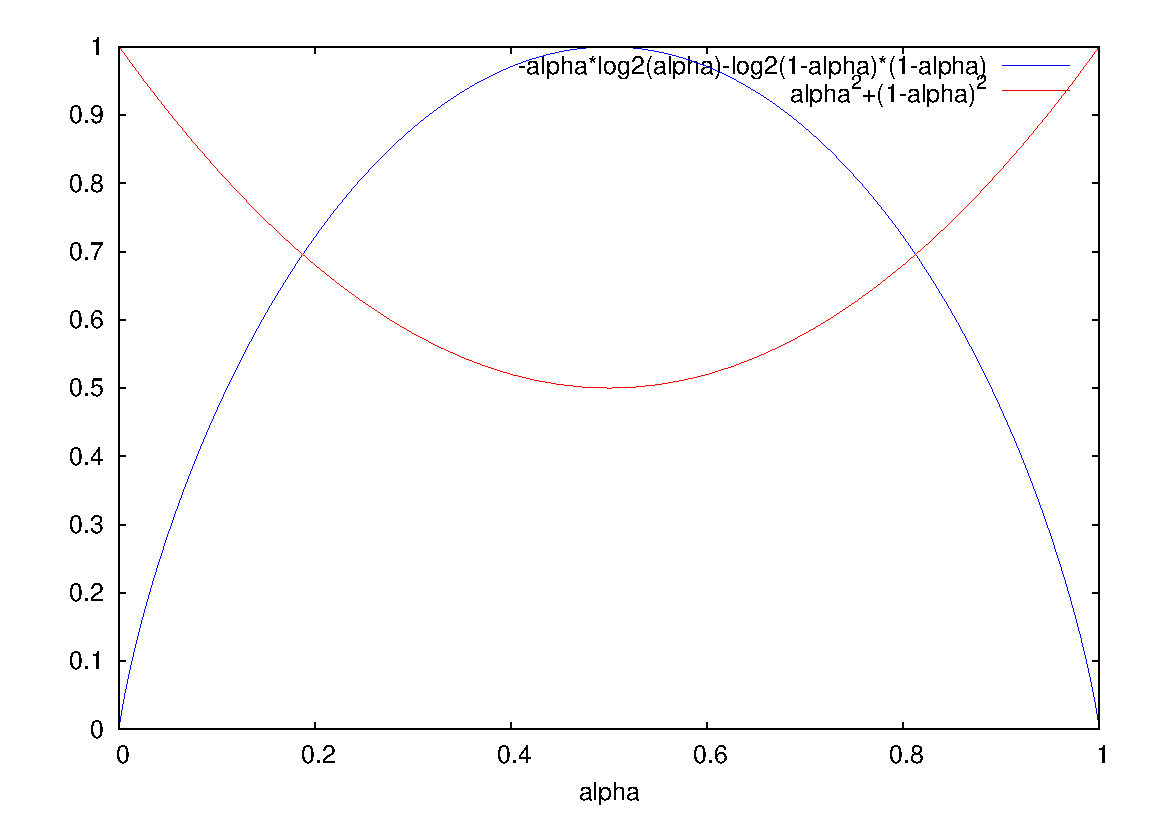
\includegraphics[width=.5\linewidth]{figs/maxout_1}
\end{dmath}
\ebm

\htmlrule
\section{More operators and functions}

The next four functions \func{pauli\_product}{i_1,\ldots,i_n},
\func{pauliexp}{\rho}, \func{invpauliexp}{c}, and \func{correlation\_tensor}{c,i_1,\ldots,i_n}
are related. An example using them follows their definitions.

\subsection{\ifs{pauli\_product} \ tensor product of pauli matrices }
\func{pauli\_product}{i_1,\ldots,i_n} returns the tensor product
$\sigma_{i_1} \otimes \cdots \otimes \sigma_{i_n}$, where the indices
$i_j$ are in $\{0,1,2,3\}$. 

\subsection{\ifs{pauliexp}\ expansion in terms of tensor products of pauli matrices  }
\func{pauliexp}{\rho} returns the correlation tensor, that
is, the coefficients in the expansion of the matrix $\rho$
in tensor products of pauli matrices. Explicitly, \fs{pauliexp}
returns the coefficents $c_{i_1,\ldots,i_n}$ in
\begin{equation}\label{pauliexp}
 \rho = \sum_{i_1,\ldots,i_n=0}^1 c_{i_1,\ldots,i_n} \ \sigma_{i_1} \otimes \cdots \otimes \sigma_{i_n}.
\end{equation}
$\rho$ must be a $2^n\times 2^n$ matrix. The coefficients are returned as a list
of $2^n\times 2^n$ elements. The place of $c_{i_1,\ldots,i_n}$ in the returned list is determined
by taking ${i_1,\ldots,i_n}$ to be the  binary representation of an integer. For convenience,
the coefficient can be retrieved by index with the function \fs{correlation\_tensor}.

\subsection{\ifs{invpauliexp} inverse of expansion in terms of tensor products of pauli matrices}
\func{invpauliexp}{c} is the inverse of \fs{pauiexp}. Given a list $c$ representing
the correlation tensor ({\it i.e.} expansion coefficients),
 \fs{invpauliexp} returns the matrix $\rho$ given by (\ref{pauliexp}).

\subsection{\fs{correlation\_tensor} retrieve component of correlation tensor by index}
\func{correlation\_tensor}{c,i_1,\ldots,i_n} returns the expansion coefficient for
the term $\sigma_{i_1} \otimes \cdots \otimes \sigma_{i_n}$ in the expansion of
$\rho$, where $c$ is the list of coefficients in the expansion of $\rho$ as given,
for intance, by \fs{pauliexp}.

\subsection{Using \fs{pauliexp} and \fs{invpauliexp}; an example}
Here is an example using the four functions defined above.
First we create three generic $2\times2$ (complex) matrices.
\bbm
\begin{verbatim}
(%i2) m1 : matrix([a1,b1],[c1,d1]);
\end{verbatim}
\begin{dmath}[number={\%o2}]
 \pmatrix{\mathrm{a1}&\linebreak[0]\mathrm{b1}\cr \mathrm{c1}&\linebreak[0]\mathrm{d1}\cr }\end{dmath}
\begin{verbatim}
(%i3) m2 : matrix([a2,b2],[c2,d2]) $
(%i4) m3 : matrix([a3,b3],[c3,d3]) $
\end{verbatim}
\ebm
Here is the tensor product of the three matrices. This is {\it not} a generic element in
the three qubit Hilbert space represented by $M(\mathbb{C},8)$. For instance,
the three matrices have $12$ complex parameters while a generic matrix in
the tensor product space  has $64$ complex parameters.
\bbm
\begin{verbatim}
(%i5) mp : m1 otimes m2 otimes  m3 ;
\end{verbatim}
\begin{dmath}[number={\%o5}]
 \pmatrix{\mathrm{a1}\*\mathrm{a2}\*\mathrm{a3}&\linebreak[0]\mathrm{a1}\*\mathrm{a2}\*\mathrm{b3}&\linebreak[0]\mathrm{a1}\*\mathrm{a3}\*\mathrm{b2}&\linebreak[0]\mathrm{a1}\*\mathrm{b2}\*\mathrm{b3}&\linebreak[0]\mathrm{a2}\*\mathrm{a3}\*\mathrm{b1}&\linebreak[0]\mathrm{a2}\*\mathrm{b1}\*\mathrm{b3}&\linebreak[0]\mathrm{a3}\*\mathrm{b1}\*\mathrm{b2}&\linebreak[0]\mathrm{b1}\*\mathrm{b2}\*\mathrm{b3}\cr \mathrm{a1}\*\mathrm{a2}\*\mathrm{c3}&\linebreak[0]\mathrm{a1}\*\mathrm{a2}\*\mathrm{d3}&\linebreak[0]\mathrm{a1}\*\mathrm{b2}\*\mathrm{c3}&\linebreak[0]\mathrm{a1}\*\mathrm{b2}\*\mathrm{d3}&\linebreak[0]\mathrm{a2}\*\mathrm{b1}\*\mathrm{c3}&\linebreak[0]\mathrm{a2}\*\mathrm{b1}\*\mathrm{d3}&\linebreak[0]\mathrm{b1}\*\mathrm{b2}\*\mathrm{c3}&\linebreak[0]\mathrm{b1}\*\mathrm{b2}\*\mathrm{d3}\cr \mathrm{a1}\*\mathrm{a3}\*\mathrm{c2}&\linebreak[0]\mathrm{a1}\*\mathrm{b3}\*\mathrm{c2}&\linebreak[0]\mathrm{a1}\*\mathrm{a3}\*\mathrm{d2}&\linebreak[0]\mathrm{a1}\*\mathrm{b3}\*\mathrm{d2}&\linebreak[0]\mathrm{a3}\*\mathrm{b1}\*\mathrm{c2}&\linebreak[0]\mathrm{b1}\*\mathrm{b3}\*\mathrm{c2}&\linebreak[0]\mathrm{a3}\*\mathrm{b1}\*\mathrm{d2}&\linebreak[0]\mathrm{b1}\*\mathrm{b3}\*\mathrm{d2}\cr \mathrm{a1}\*\mathrm{c2}\*\mathrm{c3}&\linebreak[0]\mathrm{a1}\*\mathrm{c2}\*\mathrm{d3}&\linebreak[0]\mathrm{a1}\*\mathrm{c3}\*\mathrm{d2}&\linebreak[0]\mathrm{a1}\*\mathrm{d2}\*\mathrm{d3}&\linebreak[0]\mathrm{b1}\*\mathrm{c2}\*\mathrm{c3}&\linebreak[0]\mathrm{b1}\*\mathrm{c2}\*\mathrm{d3}&\linebreak[0]\mathrm{b1}\*\mathrm{c3}\*\mathrm{d2}&\linebreak[0]\mathrm{b1}\*\mathrm{d2}\*\mathrm{d3}\cr \mathrm{a2}\*\mathrm{a3}\*\mathrm{c1}&\linebreak[0]\mathrm{a2}\*\mathrm{b3}\*\mathrm{c1}&\linebreak[0]\mathrm{a3}\*\mathrm{b2}\*\mathrm{c1}&\linebreak[0]\mathrm{b2}\*\mathrm{b3}\*\mathrm{c1}&\linebreak[0]\mathrm{a2}\*\mathrm{a3}\*\mathrm{d1}&\linebreak[0]\mathrm{a2}\*\mathrm{b3}\*\mathrm{d1}&\linebreak[0]\mathrm{a3}\*\mathrm{b2}\*\mathrm{d1}&\linebreak[0]\mathrm{b2}\*\mathrm{b3}\*\mathrm{d1}\cr \mathrm{a2}\*\mathrm{c1}\*\mathrm{c3}&\linebreak[0]\mathrm{a2}\*\mathrm{c1}\*\mathrm{d3}&\linebreak[0]\mathrm{b2}\*\mathrm{c1}\*\mathrm{c3}&\linebreak[0]\mathrm{b2}\*\mathrm{c1}\*\mathrm{d3}&\linebreak[0]\mathrm{a2}\*\mathrm{c3}\*\mathrm{d1}&\linebreak[0]\mathrm{a2}\*\mathrm{d1}\*\mathrm{d3}&\linebreak[0]\mathrm{b2}\*\mathrm{c3}\*\mathrm{d1}&\linebreak[0]\mathrm{b2}\*\mathrm{d1}\*\mathrm{d3}\cr \mathrm{a3}\*\mathrm{c1}\*\mathrm{c2}&\linebreak[0]\mathrm{b3}\*\mathrm{c1}\*\mathrm{c2}&\linebreak[0]\mathrm{a3}\*\mathrm{c1}\*\mathrm{d2}&\linebreak[0]\mathrm{b3}\*\mathrm{c1}\*\mathrm{d2}&\linebreak[0]\mathrm{a3}\*\mathrm{c2}\*\mathrm{d1}&\linebreak[0]\mathrm{b3}\*\mathrm{c2}\*\mathrm{d1}&\linebreak[0]\mathrm{a3}\*\mathrm{d1}\*\mathrm{d2}&\linebreak[0]\mathrm{b3}\*\mathrm{d1}\*\mathrm{d2}\cr \mathrm{c1}\*\mathrm{c2}\*\mathrm{c3}&\linebreak[0]\mathrm{c1}\*\mathrm{c2}\*\mathrm{d3}&\linebreak[0]\mathrm{c1}\*\mathrm{c3}\*\mathrm{d2}&\linebreak[0]\mathrm{c1}\*\mathrm{d2}\*\mathrm{d3}&\linebreak[0]\mathrm{c2}\*\mathrm{c3}\*\mathrm{d1}&\linebreak[0]\mathrm{c2}\*\mathrm{d1}\*\mathrm{d3}&\linebreak[0]\mathrm{c3}\*\mathrm{d1}\*\mathrm{d2}&\linebreak[0]\mathrm{d1}\*\mathrm{d2}\*\mathrm{d3}\cr }\end{dmath}
\ebm
We compute the correlation tensor of \verb|mp|
\bbm
\begin{verbatim}
(%i6) pe : pauliexp(mp) $
\end{verbatim}
\ebm
Check that the tensor has $64$ elements and see what a coefficient looks like.
\bbm
\begin{verbatim}
(%i7) length(pe);
\end{verbatim}
\begin{dmath}[number={\%o7}]
 64\end{dmath}
\begin{verbatim}
(%i8) part(pe,10);
\end{verbatim}
\begin{dmath}[number={\%o8}]
 \ifracn{-i\*\mathrm{c1}\*\mathrm{c2}\*\mathrm{d3}-i\*\mathrm{b1}\*\mathrm{c2}\*\mathrm{d3}+i\*\mathrm{b2}\*\mathrm{c1}\*\mathrm{d3}+i\*\mathrm{b1}\*\mathrm{b2}\*\mathrm{d3}-i\*\mathrm{a3}\*\mathrm{c1}\*\mathrm{c2}-i\*\mathrm{a3}\*\mathrm{b1}\*\mathrm{c2}+i\*\mathrm{a3}\*\mathrm{b2}\*\mathrm{c1}+i\*\mathrm{a3}\*\mathrm{b1}\*\mathrm{b2}}{8}\end{dmath}
\ebm
Check that the inverse of the expansion gives the original matrix back
\bbm
\begin{verbatim}
(%i9) is ( ratsimp( invpauliexp( pauliexp(mp) )) = mp);
\end{verbatim}
\begin{dmath}[number={\%o9}]
 \mathbf{true}\end{dmath}
\ebm
Here is the convenience function to return an element of the correlation tensor by index
\bbm
\begin{verbatim}
(%i10) correlation_tensor(pe,1,2,3);
\end{verbatim}
\begin{dmath}[number={\%o10}]
 \ifracn{i\*\mathrm{c1}\*\mathrm{c2}\*\mathrm{d3}+i\*\mathrm{b1}\*\mathrm{c2}\*\mathrm{d3}-i\*\mathrm{b2}\*\mathrm{c1}\*\mathrm{d3}-i\*\mathrm{b1}\*\mathrm{b2}\*\mathrm{d3}-i\*\mathrm{a3}\*\mathrm{c1}\*\mathrm{c2}-i\*\mathrm{a3}\*\mathrm{b1}\*\mathrm{c2}+i\*\mathrm{a3}\*\mathrm{b2}\*\mathrm{c1}+i\*\mathrm{a3}\*\mathrm{b1}\*\mathrm{b2}}{8}\end{dmath}
\ebm

\subsection{\ifs{fidelity}}
\func{fidelity}{\rho_1,\rho_2} returns the scalar valued fidelity
of the density matrices $\rho_1$ and $\rho_2$ defined by
$$
 \mbox{Tr}\left(\sqrt{\sqrt{\rho_2}\rho_1\sqrt{\rho_2}}\right).
$$

\subsection{\ifs{spinor\_rotation\_op}, \ifs{spinor\_rotation\_op\_trig}}
 Stub

\htmlrule
\section{Entanglement.  longer examples}

\subsection{Entanglement swapping\index{entanglement swapping}}

Consider a pair of entangled qubits $A$ and $B$, and another
entangled pair $C$ and $D$. By performing a joint
measurement on, say $B$ and $C$, we can put $A$ and $B$ in
an entangled state although they may be widely separated.
We begin by considering the most general projective measure
on $B$ and $C$, and calculate the reduced density matrix for
a single qubit and the probability of outcome. In this
example we calculate these quantities two ways--- one,
directly from the density matrix formalism, and two, via
formulas taking advantage of the particulars of this
problem. To do the first calculation by hand would be
extremely upleasant, as it involves multiplying $16\times16$
matrices with several factors in a single element. Carrying
it out below with \pname{Maxima} is a concise exercise. This
may appear to be an empty exercise only because all the
calculations agree. In fact, in taking this example from a
journal article, the author easily found a typographical
error leading to an inconsistent result in one of the
formulas below that would have been difficult to track down
by hand. At present this example does not continue by discussing
the measurements that maximize the resulting entanglement
of $A$ and $D$.

Qubits $A$ and $B$ are in the state
$$
\ket{\alpha}=\sqrt{\alpha}\ket{00}+ \sqrt{1-\alpha}\ket{11},
$$
$C$ and $D$ are in the state
$$
\ket{\beta}=\sqrt{\beta}\ket{00}+ \sqrt{1-\beta}\ket{11},
$$
with the Schmidt coefficients \index{Schmidt coefficients}
satisfying $\alpha,\beta >1/2$.
For now, we only want to tell \pname{Maxima} that the coefficients
of the kets are real.\ibd{assume}
 \bbm
\begin{verbatim}
(%i2) assume(alpha>0,1-alpha>0,beta>0,1-beta>0);
\end{verbatim}
\begin{dmath}[number={\%o2}]
 \left[ \alpha>0,\linebreak[0]\alpha<1,\linebreak[0]\beta>0,\linebreak[0]\beta<1 \right] \end{dmath}
\begin{verbatim}
(%i3) a : schmidt_ket(alpha);
\end{verbatim}
\begin{dmath}[number={\%o3}]
 \pmatrix{\isqrt{\alpha}\cr 0\cr 0\cr \isqrt{1-\alpha}\cr }\end{dmath}
\begin{verbatim}
(%i4) b : schmidt_ket(beta);
\end{verbatim}
\begin{dmath}[number={\%o4}]
 \pmatrix{\isqrt{\beta}\cr 0\cr 0\cr \isqrt{1-\beta}\cr }\end{dmath}
\ebm
We consider the projective measurement\index{projective measure} $\{E_m\}$, that is $E_m=\ket{u_m}\bra{u_m}$
and $\sum_m E_m=\mathbb{1}_4$. We consider only a single basis vector
here, so we don't use the subscript $m$ for \pname{Maxima} vector name.
We need to use \pname{Maxima}'s \ifs{declare} to declare that 
the components are complex. \index{complex numbers!declaring variable complex}
The state $\ket{u_m}$ is normalized, but we don't need to impose that condition in
\pname{Maxima} at this point.
\bbm
\begin{verbatim}
(%i5)  declare([u00,u01,u10,u11], complex);
\end{verbatim}
\begin{dmath}[number={\%o5}]
 \mathbf{done}\end{dmath}
\begin{verbatim}
(%i6) u : ket(u00,u01,u10,u11);
\end{verbatim}
\begin{dmath}[number={\%o6}]
 \pmatrix{\mathrm{u00}\cr \mathrm{u01}\cr \mathrm{u10}\cr \mathrm{u11}\cr }\end{dmath}
\ebm
The inital joint state $\ket{\alpha\beta}\bra{\alpha\beta}$ is pure and remains
so after the measurment applying $\ket{u_m}\bra{u_m}$ to qubits $B$ and $C$.
But we write the density operator
because we will examine the reduced states, which are mixed.
\bbm
\begin{verbatim}
(%i7) rho : conjsimp((ident(2) otimes toproj(u) otimes ident(2)) . toproj(a otimes b))$,
\end{verbatim}
\ebm
where \ifs{conjsimp} 
(supplied via the \pname{Maxima} listserv by Barton Willis) replaces $xx^*$ with $|x|^2$.
The output was suppressed with the trailing dollar sign because the $\rho$ is
a $16\times16$ matrix with large expressions for entries.
%\everymath{\scriptscriptstyle}
%\newcommand{\myrm}[1]{\scriptscriptstyle{#1}}
%\newcommand{\mylineb}{\scriptscriptstyle \linebreak[0] \scriptscriptstyle }
%\newcommand{\myalpha}{\scriptscriptstyle \alpha }
%\newcommand{\myisqrt}[1]{\scriptscriptstyle\sqrt{#1}}
The reduced state of qubits $A$ and $D$ is obtained by tracing out components $2$ and
$3$ corresponding to qubits $B$ and $C$, ie  $\rho_{AD} =\mbox{Tr}_{BC}\rho$.
\ibd{ptrace}
\bbm
\begin{verbatim}
(%i8) rho_14 : ptrace(rho,2,3);
\end{verbatim}
\begin{dmath}[number={\%o8},style={\tiny}]
 \pmatrix{\alpha\*\beta\*\left| \mathrm{u00}\right| ^{2}&\linebreak[0]\alpha\*\isqrt{1-\beta}\*\isqrt{\beta}\*\mathrm{u00}^{\star}\*\mathrm{u01}&\linebreak[0]\isqrt{1-\alpha}\*\isqrt{\alpha}\*\beta\*\mathrm{u00}^{\star}\*\mathrm{u10}&\linebreak[0]\isqrt{1-\alpha}\*\isqrt{\alpha}\*\isqrt{1-\beta}\*\isqrt{\beta}\*\mathrm{u00}^{\star}\*\mathrm{u11}\cr \alpha\*\isqrt{1-\beta}\*\isqrt{\beta}\*\mathrm{u00}\*\mathrm{u01}^{\star}&\linebreak[0]\left(\alpha-\alpha\*\beta\right)\*\left| \mathrm{u01}\right| ^{2}&\linebreak[0]\isqrt{1-\alpha}\*\isqrt{\alpha}\*\isqrt{1-\beta}\*\isqrt{\beta}\*\mathrm{u01}^{\star}\*\mathrm{u10}&\linebreak[0]\left(\isqrt{1-\alpha}\*\isqrt{\alpha}-\isqrt{1-\alpha}\*\isqrt{\alpha}\*\beta\right)\*\mathrm{u01}^{\star}\*\mathrm{u11}\cr \isqrt{1-\alpha}\*\isqrt{\alpha}\*\beta\*\mathrm{u00}\*\mathrm{u10}^{\star}&\linebreak[0]\isqrt{1-\alpha}\*\isqrt{\alpha}\*\isqrt{1-\beta}\*\isqrt{\beta}\*\mathrm{u01}\*\mathrm{u10}^{\star}&\linebreak[0]\left(1-\alpha\right)\*\beta\*\left| \mathrm{u10}\right| ^{2}&\linebreak[0]\left(1-\alpha\right)\*\isqrt{1-\beta}\*\isqrt{\beta}\*\mathrm{u10}^{\star}\*\mathrm{u11}\cr \isqrt{1-\alpha}\*\isqrt{\alpha}\*\isqrt{1-\beta}\*\isqrt{\beta}\*\mathrm{u00}\*\mathrm{u11}^{\star}&\linebreak[0]\left(\isqrt{1-\alpha}\*\isqrt{\alpha}-\isqrt{1-\alpha}\*\isqrt{\alpha}\*\beta\right)\*\mathrm{u01}\*\mathrm{u11}^{\star}&\linebreak[0]\left(1-\alpha\right)\*\isqrt{1-\beta}\*\isqrt{\beta}\*\mathrm{u10}\*\mathrm{u11}^{\star}&\linebreak[0]\left(\left(\alpha-1\right)\*\beta-\alpha+1\right)\*\left| \mathrm{u11}\right| ^{2}\cr }\end{dmath}
\ebm
Likewise, the reduced state of just qubit $D$ is
$\rho_{D} =\mbox{Tr}_{ABC}\rho$.\ibd{ptrace}\index{reduced state}
\bbm
\begin{verbatim}
(%i9) rho_4 : ptrace(rho,1,2,3);
\end{verbatim}
\begin{dmath}[number={\%o9}]
 \pmatrix{\left(1-\alpha\right)\*\beta\*\left| \mathrm{u10}\right| ^{2}+\alpha\*\beta\*\left| \mathrm{u00}\right| ^{2}&\linebreak[0]\left(1-\alpha\right)\*\isqrt{1-\beta}\*\isqrt{\beta}\*\mathrm{u10}^{\star}\*\mathrm{u11}+\alpha\*\isqrt{1-\beta}\*\isqrt{\beta}\*\mathrm{u00}^{\star}\*\mathrm{u01}\cr \left(1-\alpha\right)\*\isqrt{1-\beta}\*\isqrt{\beta}\*\mathrm{u10}\*\mathrm{u11}^{\star}+\alpha\*\isqrt{1-\beta}\*\isqrt{\beta}\*\mathrm{u00}\*\mathrm{u01}^{\star}&\linebreak[0]\left(\left(\alpha-1\right)\*\beta-\alpha+1\right)\*\left| \mathrm{u11}\right| ^{2}+\left(\alpha-\alpha\*\beta\right)\*\left| \mathrm{u01}\right| ^{2}\cr }\end{dmath}
\ebm
The second method of calculating $\rho_{D}$ is as follows.
Considering the following map from
$\mathbb{C}^2\otimes\mathbb{C}^2$ to $M(\mathbb{C},2)$:
\begin{equation}\label{ket_to_mat}
    \ket{a}=\sum_{i,j=0}^1 a_{ij}\ket{ij}\quad\mapsto\quad\widehat{a}=
    \pmatrix{
      a_{00} & a_{01} \cr
      a_{10} & a_{11} \cr
    },
\end{equation}
one can show that $\rho_{D}$ is equal to $X_m^{}X_m^{\dagger}$, with
$X_m = \widehat{\alpha}\,\widehat{u}_m\,\widehat{\beta}$.
The \pname{Maxima} function implementing the mapping (\ref{ket_to_mat}) is
\bbm
\begin{verbatim}
(%i10) ket_to_mat(iket) := matrix([iket[1,1],iket[2,1]],[iket[3,1],iket[4,1]])$
\end{verbatim}
\ebm
Then the second calculation of $\rho_D$, which we call \verb|rho_4a| is given by
the following two lines.
\bbm
\begin{verbatim}
(%i11)  X : ket_to_mat(a) . ket_to_mat(u) . ket_to_mat(b);
\end{verbatim}
\begin{dmath}[number={\%o11}]
  \pmatrix{\isqrt{\alpha}\*\isqrt{\beta}\*\mathrm{u00}&\linebreak[0]\isqrt{\alpha}\*\isqrt{1-\beta}\*\mathrm{u01}\cr
    \isqrt{1-\alpha}\*\isqrt{\beta}\*\mathrm{u10}&\linebreak[0]\isqrt{1-\alpha}\*\isqrt{1-\beta}\*\mathrm{u11}\cr
  }\end{dmath} \ibd{conjsimp}\ibd{ctranspose}
\begin{verbatim}
(%i12) rho_4a : conjsimp(ctranspose(X) . X);
\end{verbatim}
\begin{dmath}[number={\%o12}]
 \pmatrix{\left(1-\alpha\right)\*\beta\*\left| \mathrm{u10}\right| ^{2}+\alpha\*\beta\*\left| \mathrm{u00}\right| ^{2}&\linebreak[0]\left(1-\alpha\right)\*\isqrt{1-\beta}\*\isqrt{\beta}\*\mathrm{u10}^{\star}\*\mathrm{u11}+\alpha\*\isqrt{1-\beta}\*\isqrt{\beta}\*\mathrm{u00}^{\star}\*\mathrm{u01}\cr \left(1-\alpha\right)\*\isqrt{1-\beta}\*\isqrt{\beta}\*\mathrm{u10}\*\mathrm{u11}^{\star}+\alpha\*\isqrt{1-\beta}\*\isqrt{\beta}\*\mathrm{u00}\*\mathrm{u01}^{\star}&\linebreak[0]\left(\left(\alpha-1\right)\*\beta-\alpha+1\right)\*\left| \mathrm{u11}\right| ^{2}+\left(\alpha-\alpha\*\beta\right)\*\left| \mathrm{u01}\right| ^{2}\cr }\end{dmath}
\ebm
Comparing \verb|(%o9)| and  \verb|(%o12)|, we see that the two methods of calculating
the reduced state for qubit $D$ after the measurement give the same result, showing that the second
method is correct. Now we compute the probability 
$p_m=\mbox{Tr}(\rho)=\mbox{Tr}(\rho_D)$
that the state is in fact projected onto $\ket{u_m}$.
\bbm
\begin{verbatim}
(%i13)  res1 : conjsimp(mat_trace(rho));
\end{verbatim}
\begin{dmath}[number={\%o13}]
 \left(\left(\alpha-1\right)\*\beta-\alpha+1\right)\*\left| \mathrm{u11}\right| ^{2}+\left(1-\alpha\right)\*\beta\*\left| \mathrm{u10}\right| ^{2}+\left(\alpha-\alpha\*\beta\right)\*\left| \mathrm{u01}\right| ^{2}+\alpha\*\beta\*\left| \mathrm{u00}\right| ^{2}\end{dmath}
\begin{verbatim}
(%i14) res2 : conjsimp(mat_trace(rho_4a));
\end{verbatim}
\begin{dmath}[number={\%o14}]
 \left(\left(\alpha-1\right)\*\beta-\alpha+1\right)\*\left| \mathrm{u11}\right| ^{2}+\left(1-\alpha\right)\*\beta\*\left| \mathrm{u10}\right| ^{2}+\left(\alpha-\alpha\*\beta\right)\*\left| \mathrm{u01}\right| ^{2}+\alpha\*\beta\*\left| \mathrm{u00}\right| ^{2}\end{dmath}
\ebm
Finally, we compare this to the trace computed by hand from the expression following (\ref{ket_to_mat}),
which is given by
\begin{equation}
 p_m=\sum^1_{i,j=0} \widehat{\alpha}_{i,j}^2 \widehat{\beta}_{i,j}^2 |\widehat{u}_{m,ij}|^2
\end{equation}
\bbm
\begin{verbatim}
(%i15) res3 : ratsimp(braz(0,0).a^2 * braz(0,0).b^2 *abs(u00)^2+ braz(0,0).a^2 * braz(1,1).b^2 * abs(u01)^2 
    +  braz(1,1).a^2 * braz(0,0).b^2 * abs(u10)^2 +  braz(1,1).a^2 * braz(1,1).b^2 * abs(u11)^2);
\end{verbatim}
\begin{dmath}[number={\%o15}]
 \left(\left(\alpha-1\right)\*\beta-\alpha+1\right)\*\left| \mathrm{u11}\right| ^{2}+\left(1-\alpha\right)\*\beta\*\left| \mathrm{u10}\right| ^{2}+\left(\alpha-\alpha\*\beta\right)\*\left| \mathrm{u01}\right| ^{2}+\alpha\*\beta\*\left| \mathrm{u00}\right| ^{2}\end{dmath}
and see that $p_m$ is the same as above--- verifying this last formula was well. 
\ebm
%\section*{Index}
\htmlrule
\printindex
\htmlrule

%\addcontentsline{toc}{section}{Index}

\end{document}
